\documentclass[xetex,mathserif,serif]{beamer}
\usepackage{polyglossia}
\setdefaultlanguage[babelshorthands=true]{russian}
\usepackage{minted}
\usepackage{tabu}
\usepackage{graphicx}

\useoutertheme{infolines}

\usepackage{fontspec}
\setmainfont{FreeSans}
\newfontfamily{\russianfonttt}{FreeSans}

\definecolor{links}{HTML}{2A1B81}
\hypersetup{colorlinks,linkcolor=,urlcolor=links}

\setbeamertemplate{blocks}[rounded][shadow=false]
\setbeamercolor*{block title alerted}{fg=red!50!black,bg=red!20}
\setbeamercolor*{block body alerted}{fg=black,bg=red!10}

\tabulinesep=0.8mm

\title{Развлекательное приложение MemDer}
\author{Александр Смирнов и Феодор Жилкин}
\date{17.05.2019г}

\begin{document}

	\frame{\titlepage}

	\begin{frame}
		\frametitle{Введение}
		\begin{figure}[h]
            \center{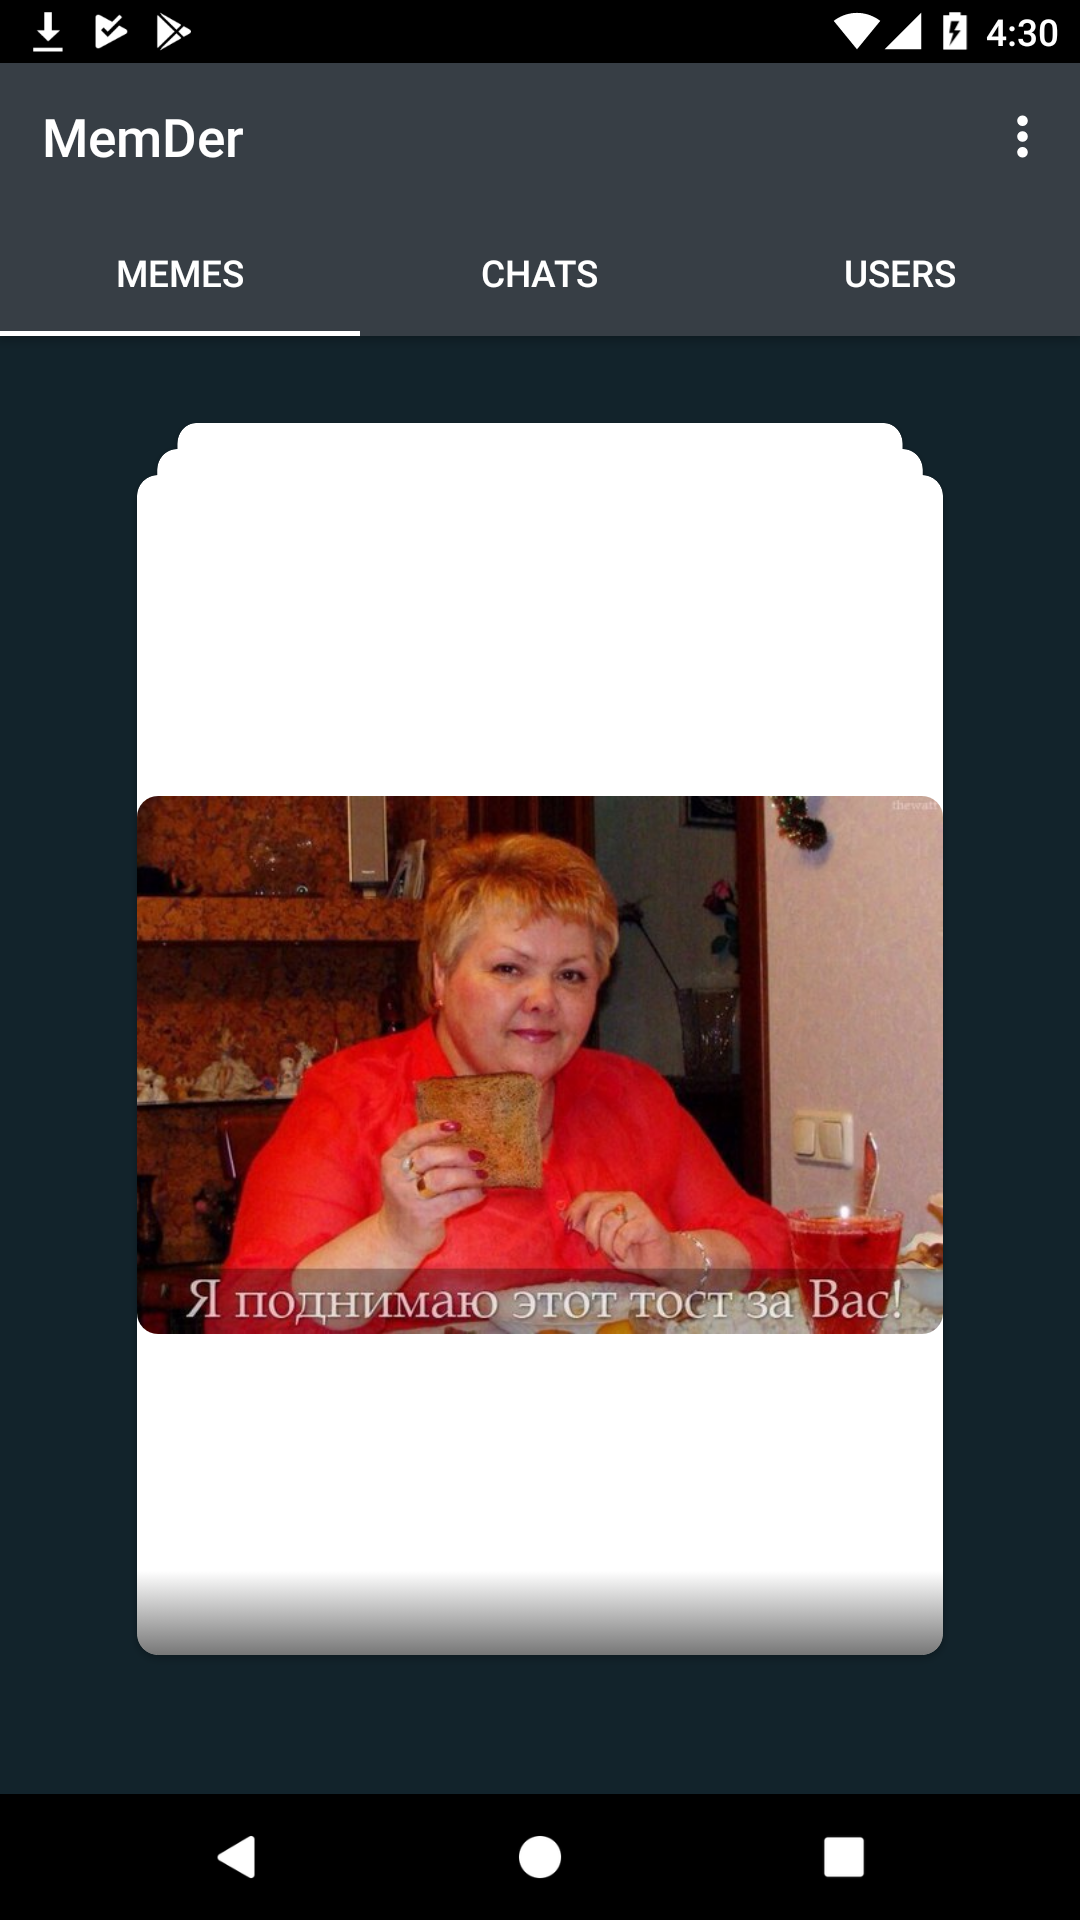
\includegraphics[scale=0.095]{images/intro.png}}
            \caption{MemDer}
            \label{fig:image}
        \end{figure}
	\end{frame}
	
	\begin{frame}
		\frametitle{Цели}
			\begin{itemize}
		 		\item Сделать законченное Android-приложение
		 		    \begin{itemize}
    			    	\item Просмотр и оценка мемов
    			    	\item Общение между пользователями
    		    	\end{itemize}
		 		\item Выложить в Google Play
				\item Получение опыта
    				\begin{itemize}
    			    	\item Фронтенд
    			    	\item Бэкенд
    			    	\item Поиск и подбор контента
    			    	\item Сервер
    		    	\end{itemize}
			\end{itemize}
	\end{frame}
	
	\begin{frame}
		\frametitle{Задачи}
			\begin{itemize}
			    \item Скрипт по скачиванию контента
		 		\item База данных мемов по категориям
				\item Чаты
				\item Регистрация и вход пользователя
				\item Удобный интерфейс для просмотра мемов
				\item Уведомления о сообщениях
				\item Составление предпочтений пользователя
					\begin{itemize}
				    	\item Подбор собеседников по предпочтениям
				    	\item Подбор контента по предпочтениям
			    	\end{itemize}
			\end{itemize}
	\end{frame}	
	
	\begin{frame}
		\frametitle{Сравнение с аналогами}
			\begin{itemize}
				\item Текстовый развлекательный контент
					\begin{itemize}
				    	\item Пикабу
				    	\item Reddit
			    	\end{itemize}
			    \item Визуальный развлекательный контент
					\begin{itemize}
				    	\item Паблики с мемами в ВК
				    	\item iFunny
			    	\end{itemize}
			\end{itemize}
	\end{frame}		
	
	\begin{frame}
		\frametitle{Интерфейс приложения (1)}
            \begin{columns}[t]
                \column{.3\textwidth}
                    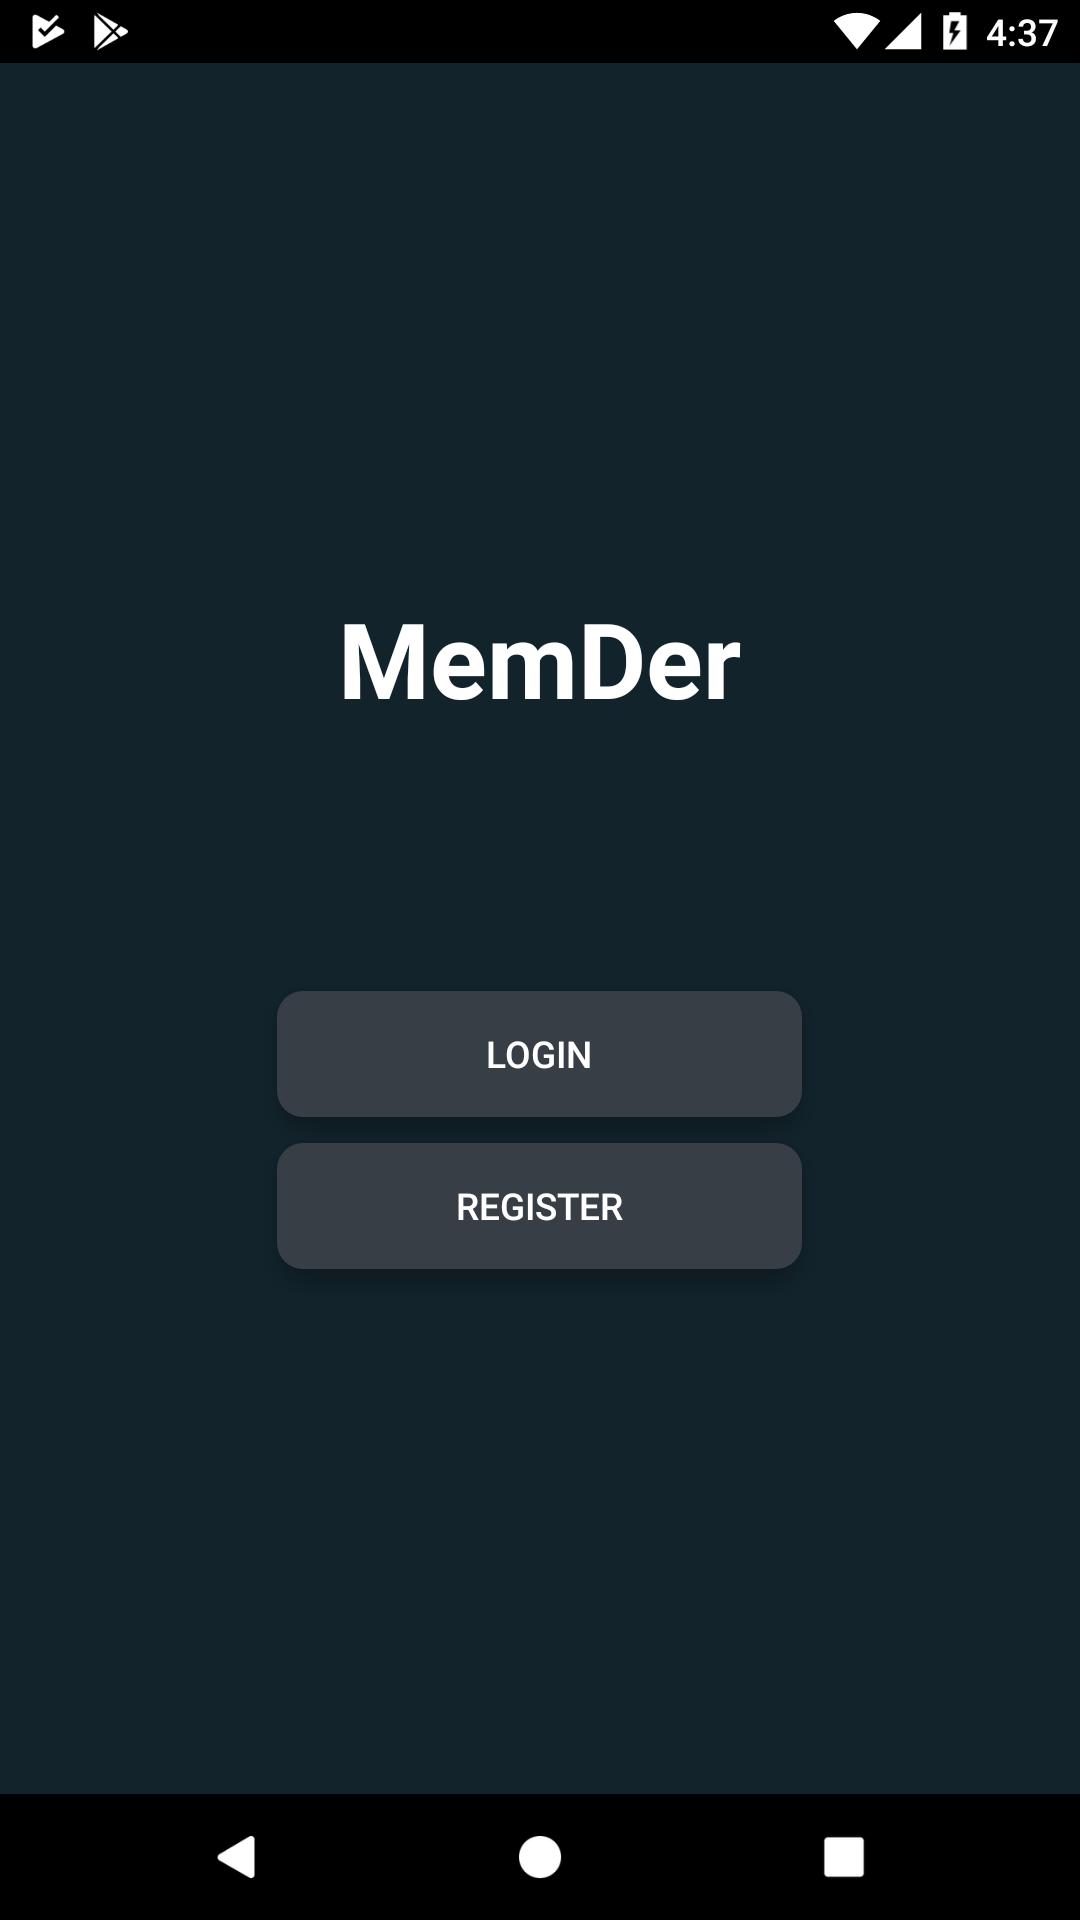
\includegraphics[scale=0.09]{images/login.png}
                \column{.3\textwidth}
                    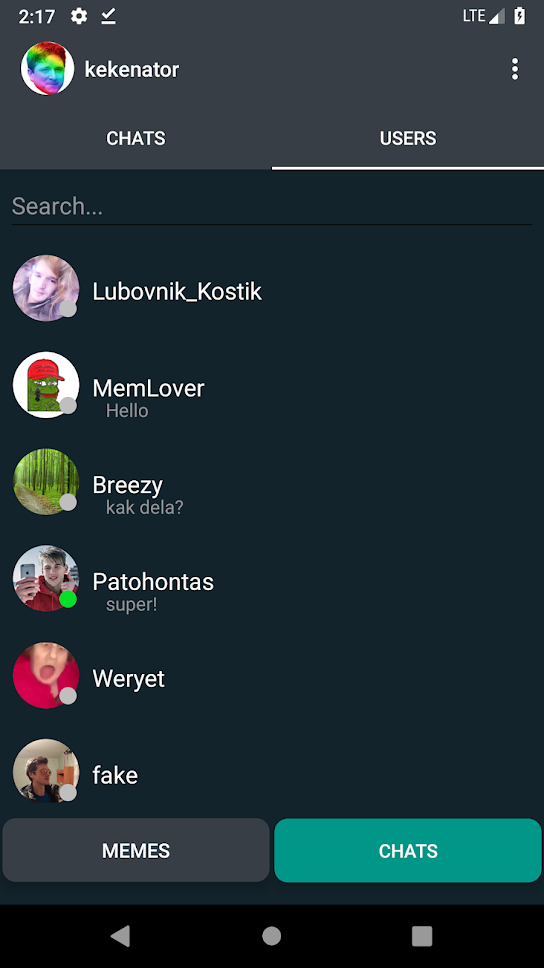
\includegraphics[scale=0.179]{images/chats.png}
                \column{.3\textwidth}
                    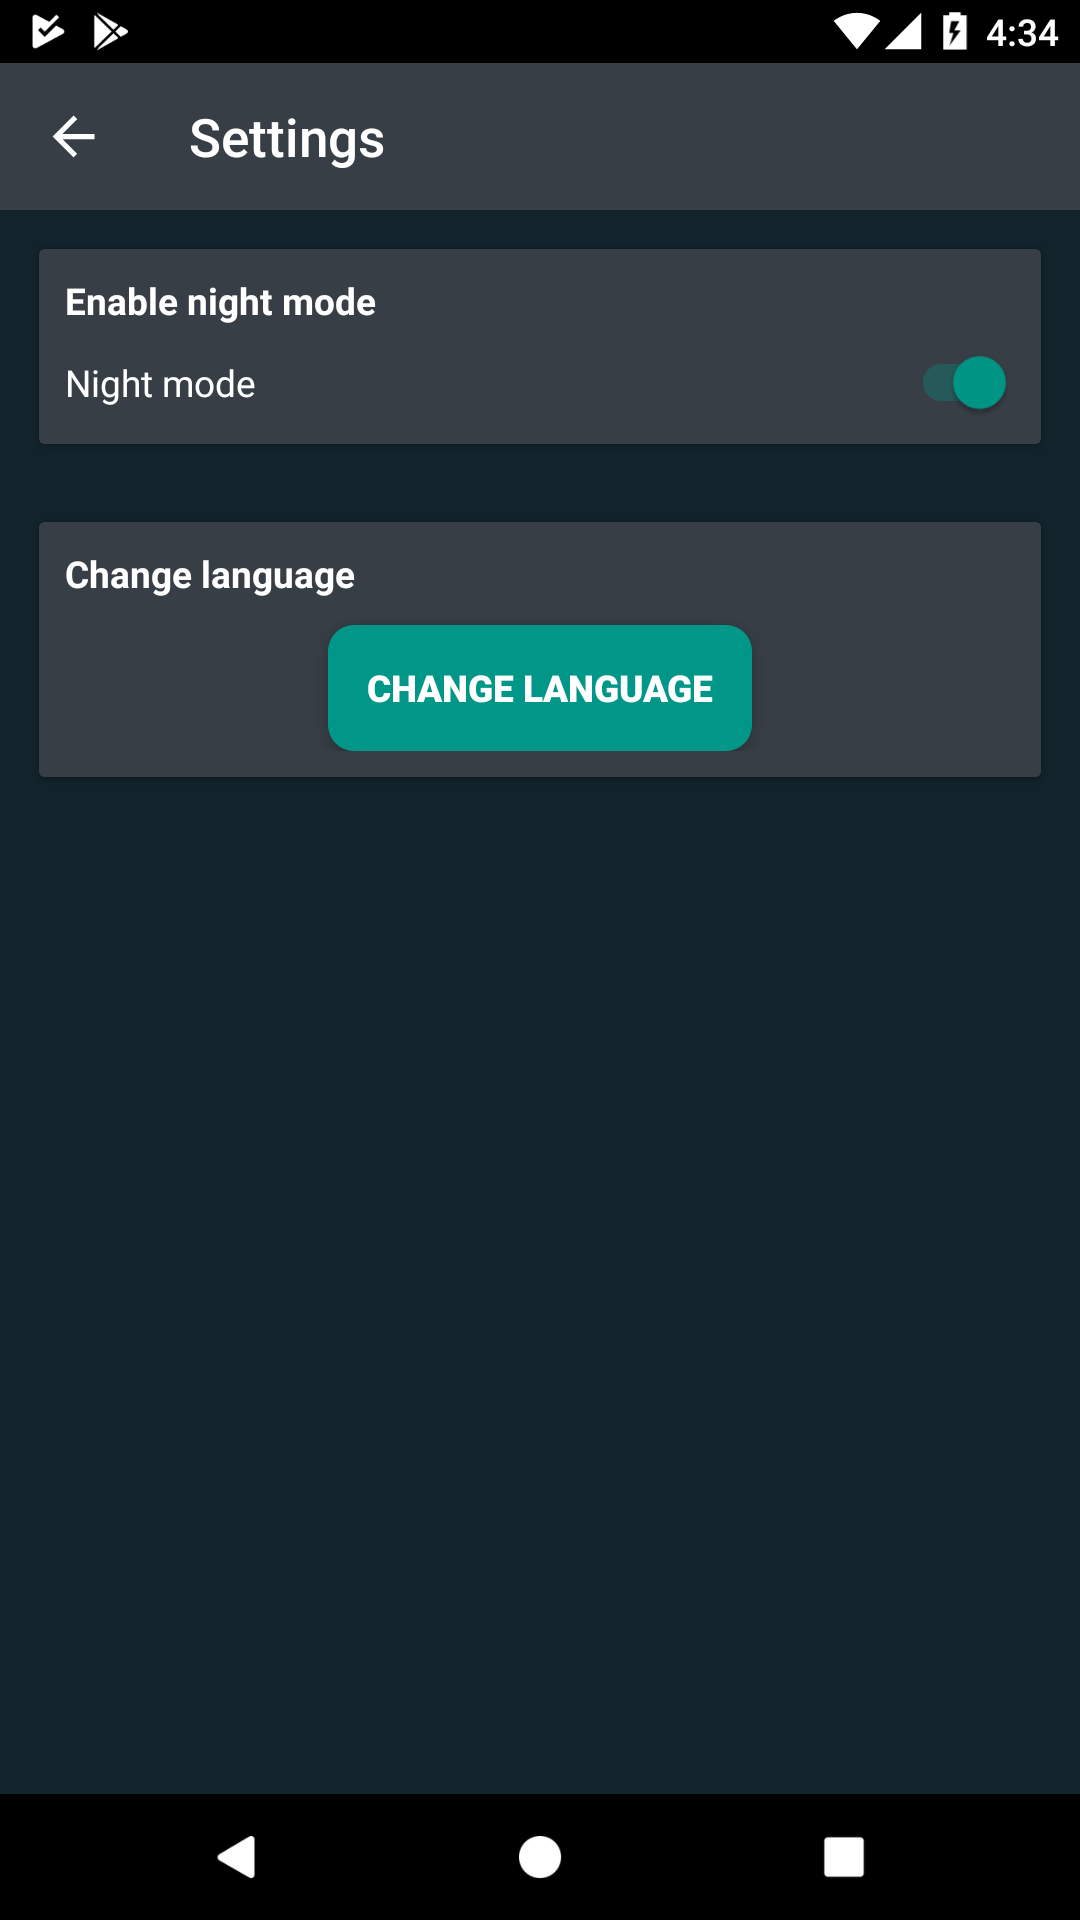
\includegraphics[scale=0.09]{images/settings.png}
                    
            \end{columns}
	\end{frame}	
	
	\begin{frame}
		\frametitle{Интерфейс приложения (2)}
		\begin{figure}[h]
            \center{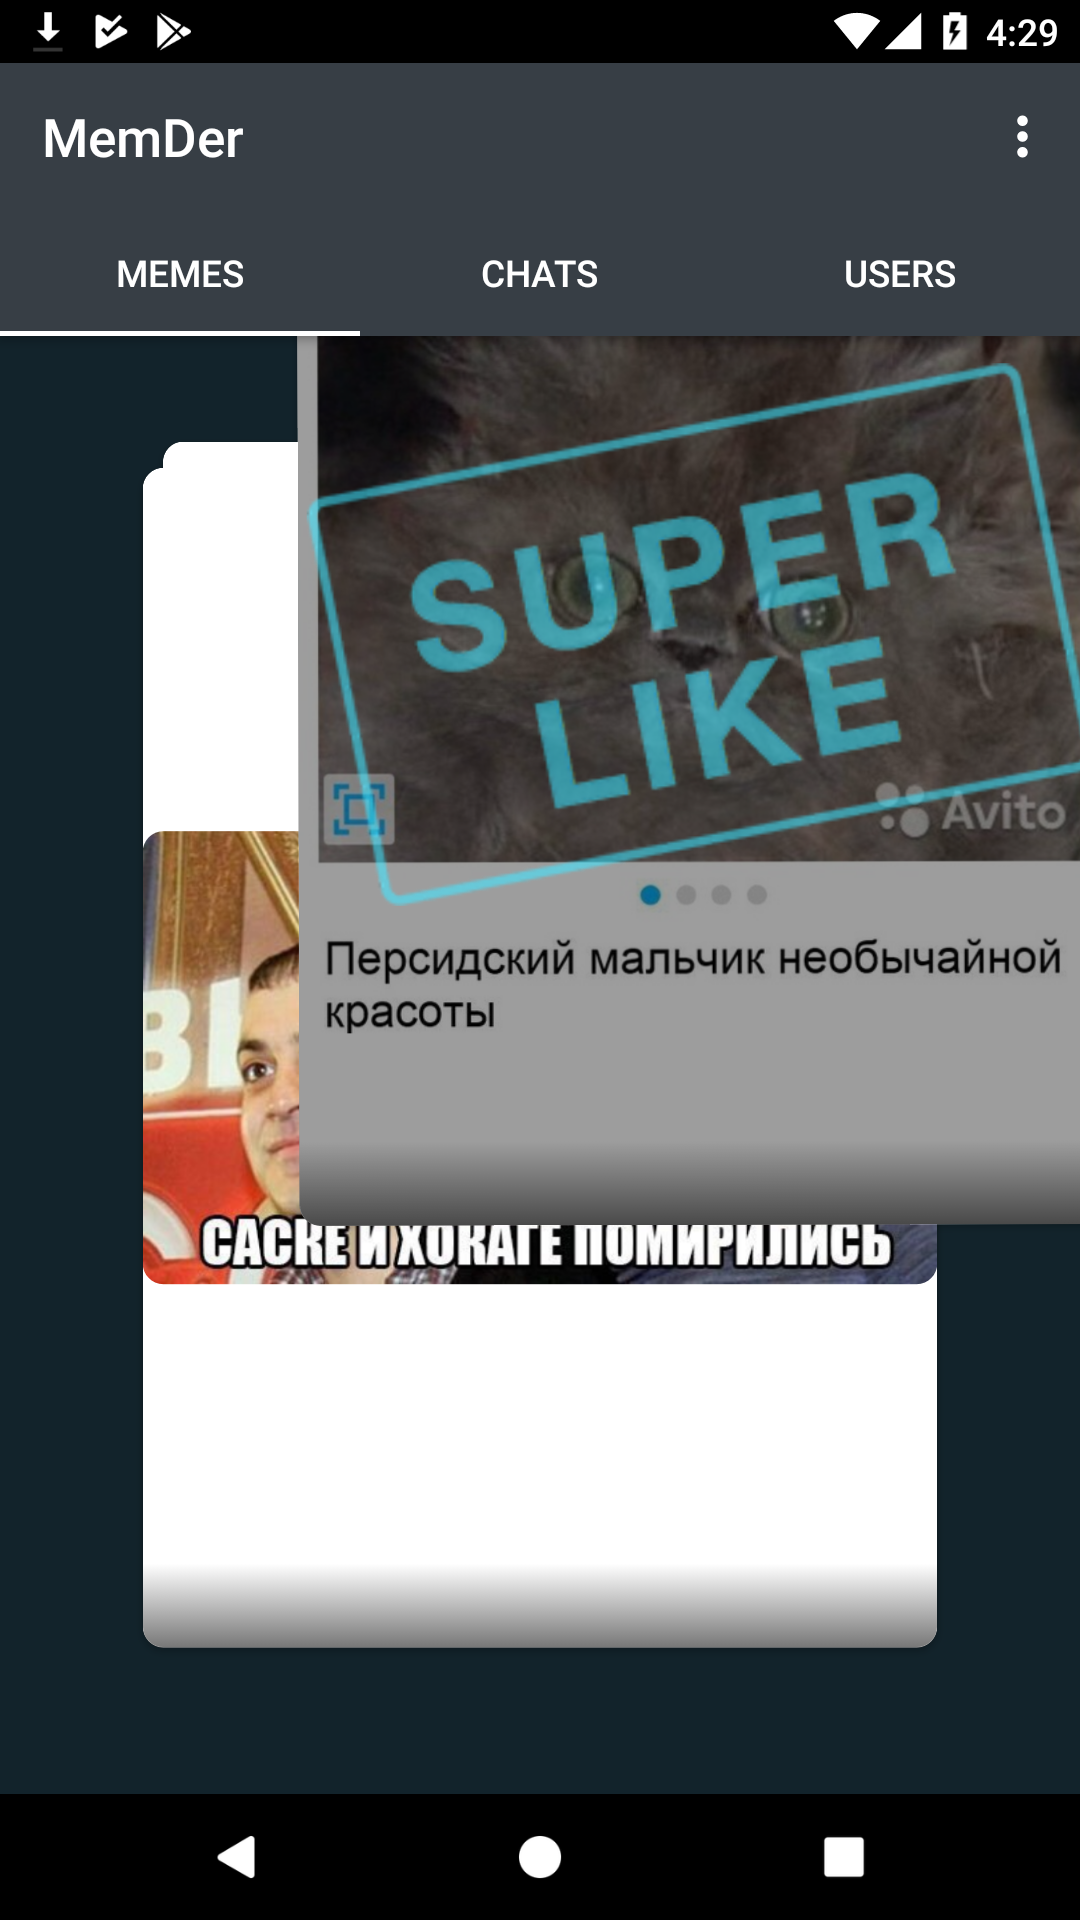
\includegraphics[scale=0.095]{images/swipe1.png}}
            \caption{MemDer}
            \label{fig:image}
        \end{figure}
	\end{frame}
	
	\begin{frame}
		\frametitle{Внутреннее устройство}
		\begin{figure}[h]
            \center{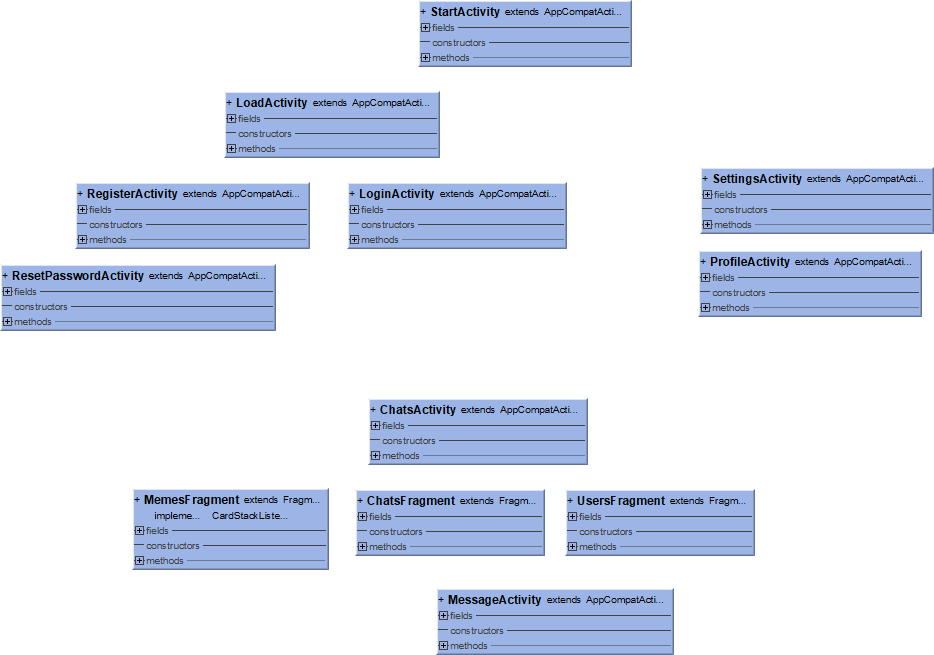
\includegraphics[scale=0.25]{images/diagram.png}}
            \caption{Диаграмма activity}
            \label{fig:image}
        \end{figure}
	\end{frame}	
	
	\begin{frame}
		\frametitle{FireBase FireStore}
		\begin{figure}[h]
            \center{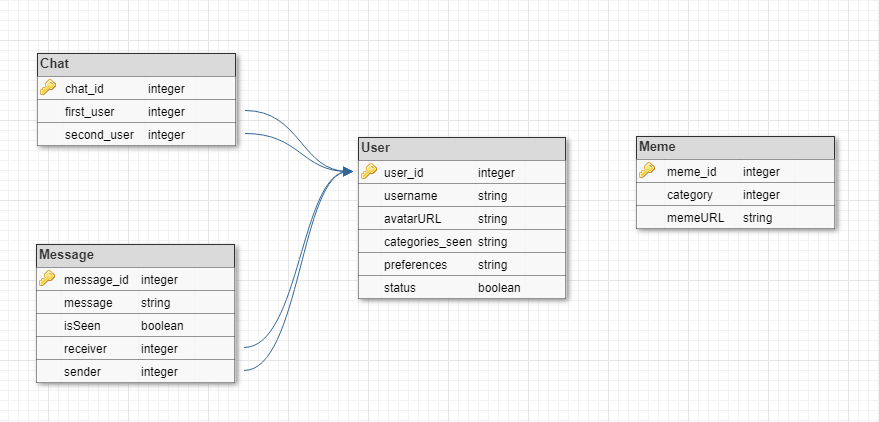
\includegraphics[scale=0.5]{images/DB.png}}
            \caption{Схема БД}
            \label{fig:image}
        \end{figure}
	\end{frame}	
	
	\begin{frame}
		\frametitle{Как это всё работает}
		\begin{figure}[h]
            \center{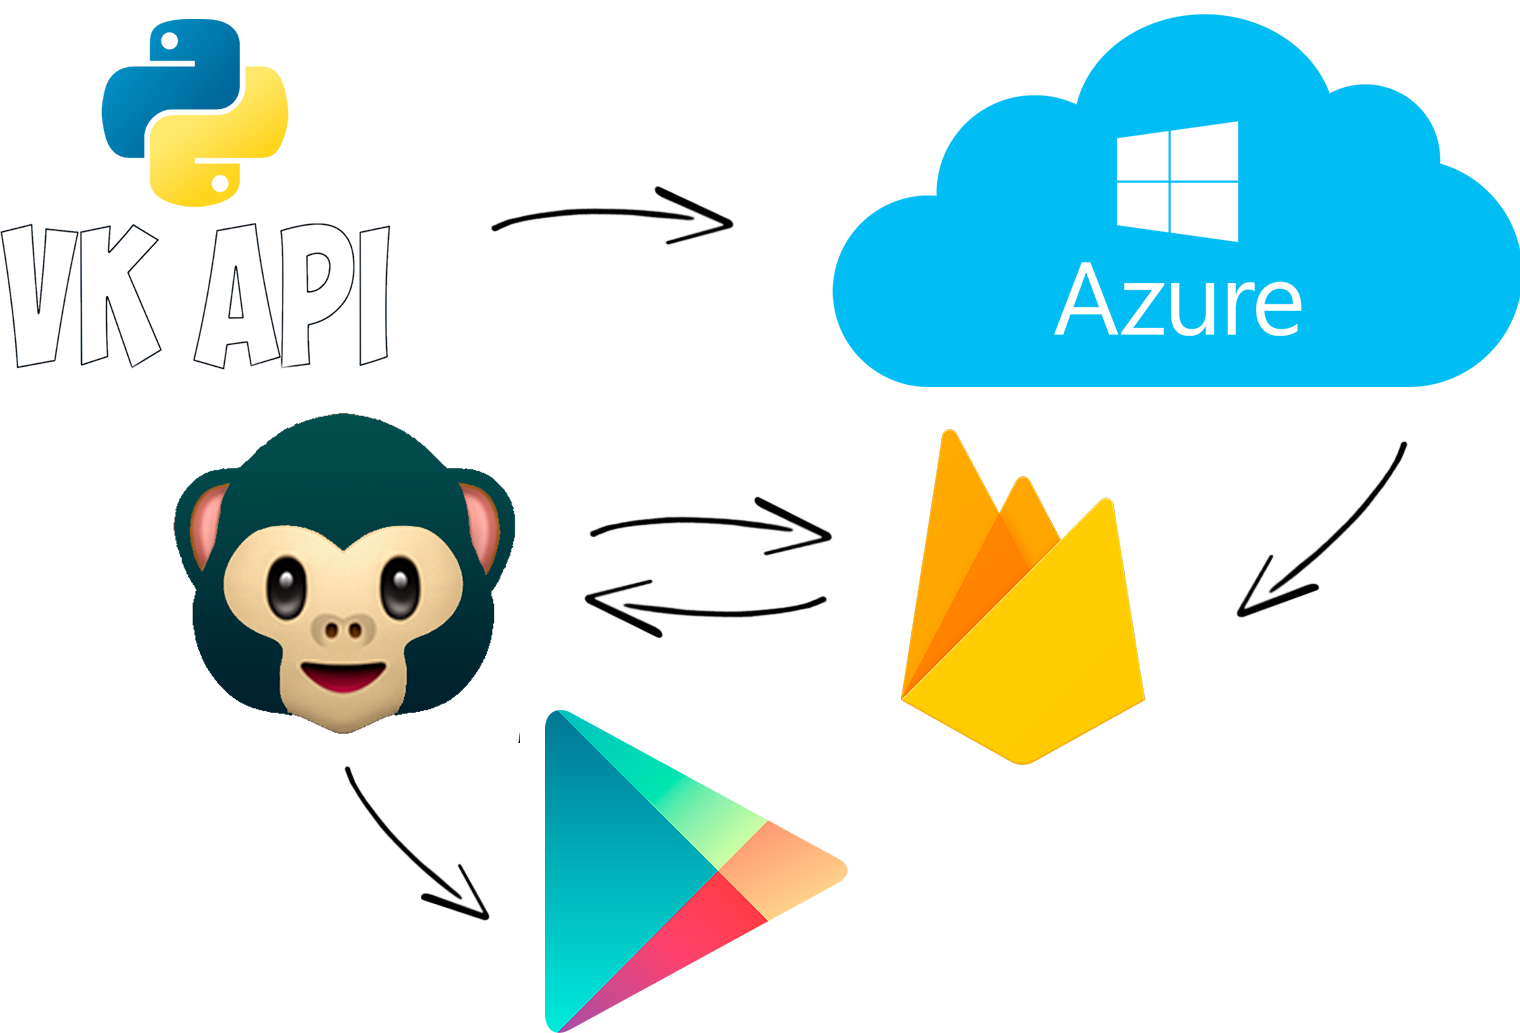
\includegraphics[scale=0.2]{images/scheme.png}}
            \caption{Схема проекта}
            \label{fig:image}
        \end{figure}
	\end{frame}	
	
	\begin{frame}
		\frametitle{Итоги}
		\begin{itemize}
			\item Александр
			    \begin{itemize}
			    	\item Чаты
			    	\item FireStore
			    	\item Алгоритм предпочтений
		        \end{itemize}
			\item Феодор
			    \begin{itemize}
			    	\item Поиск и майнинг контента
			    	\item Буфер  
			    	\item Кастомные свайпы
		        \end{itemize}
		\end{itemize}
	\end{frame}

	\begin{frame}
		\frametitle{Результаты}
		\begin{itemize}
		    \item Скрипт по скачиванию контента
			\item База данных мемов по категориям на FireBase
			\item Готовое Android-приложение, выложенное на Play Market
		    	\begin{itemize}
			    	\item Рекомендательная система для мемов
			    	\item Рекомендательная система для собеседников
			    	\item Дружелюбный интерфейс
			    	\item Чаты
			    	\item Регистрация/вход пользователя
			   	\end{itemize}
			\item Google Play — \url{https://play.google.com/store/apps/details?id=com.MemDerPack}
			\item Проект — \url{https://github.com/SmirnovAlexander/MemDer}
			\item Майнинг контента — \url{https://github.com/Feodoros/vkParser}
		\end{itemize}
	\end{frame}

\end{document}